%-------------------------------------------------------------------------------------------------------
%-------------------------------------------------------------------------------------------------------
% Sec & Label

\section{Introduction}
\label{sec:introduction}

%-------------------------------------------------------------------------------------------------------
%-------------------------------------------------------------------------------------------------------


The objective of this laboratory assignment is to create an audio amplifier circuit by choosing the architecture of the Gain and Output amplifier stages whilst optimizing the circuit on its Merit ($M$), that is given by the equation:

\[
M = \frac{voltageGain\times bandwidth}{cost\times lowerCutoffFreq}
\]

\[
 cost = cost_{resistors} + cost_{capacitors} + cost_{transistors} 
\]

$cost_{resistors} = 1MU/kOhm$; $cost_{capacitors} = 1MU/\mu F$;
$cost_{diodes} = 0.1MU/transistor$ \\

The circuit studied, displayed in figure \ref{fig:Desenho_t4} utilizes the following components:

\begin{itemize}
	\item two voltage sources ($V_1$ and $V_{cc}$)
	\item two transistors ($Q_1$,$Q_2$)
	\item six resistors ($R_1$, $R_2$, $R_e$, $R_c$, $R_{in}$, $R_{out}$)
	\item three capacitors ($C_i$, $C_b$, $C_o$,)
\end{itemize}


Theoretical and simulation analysis are presented in Section \ref{sec:analysis} and Section \ref{sec:simulation}, respectively, and the results of each are then compared.
Finally, in Section \ref{sec:conclusion} the conclusions of the laboratory assignment are outlined. 



\begin{figure}[h]
	\centering
	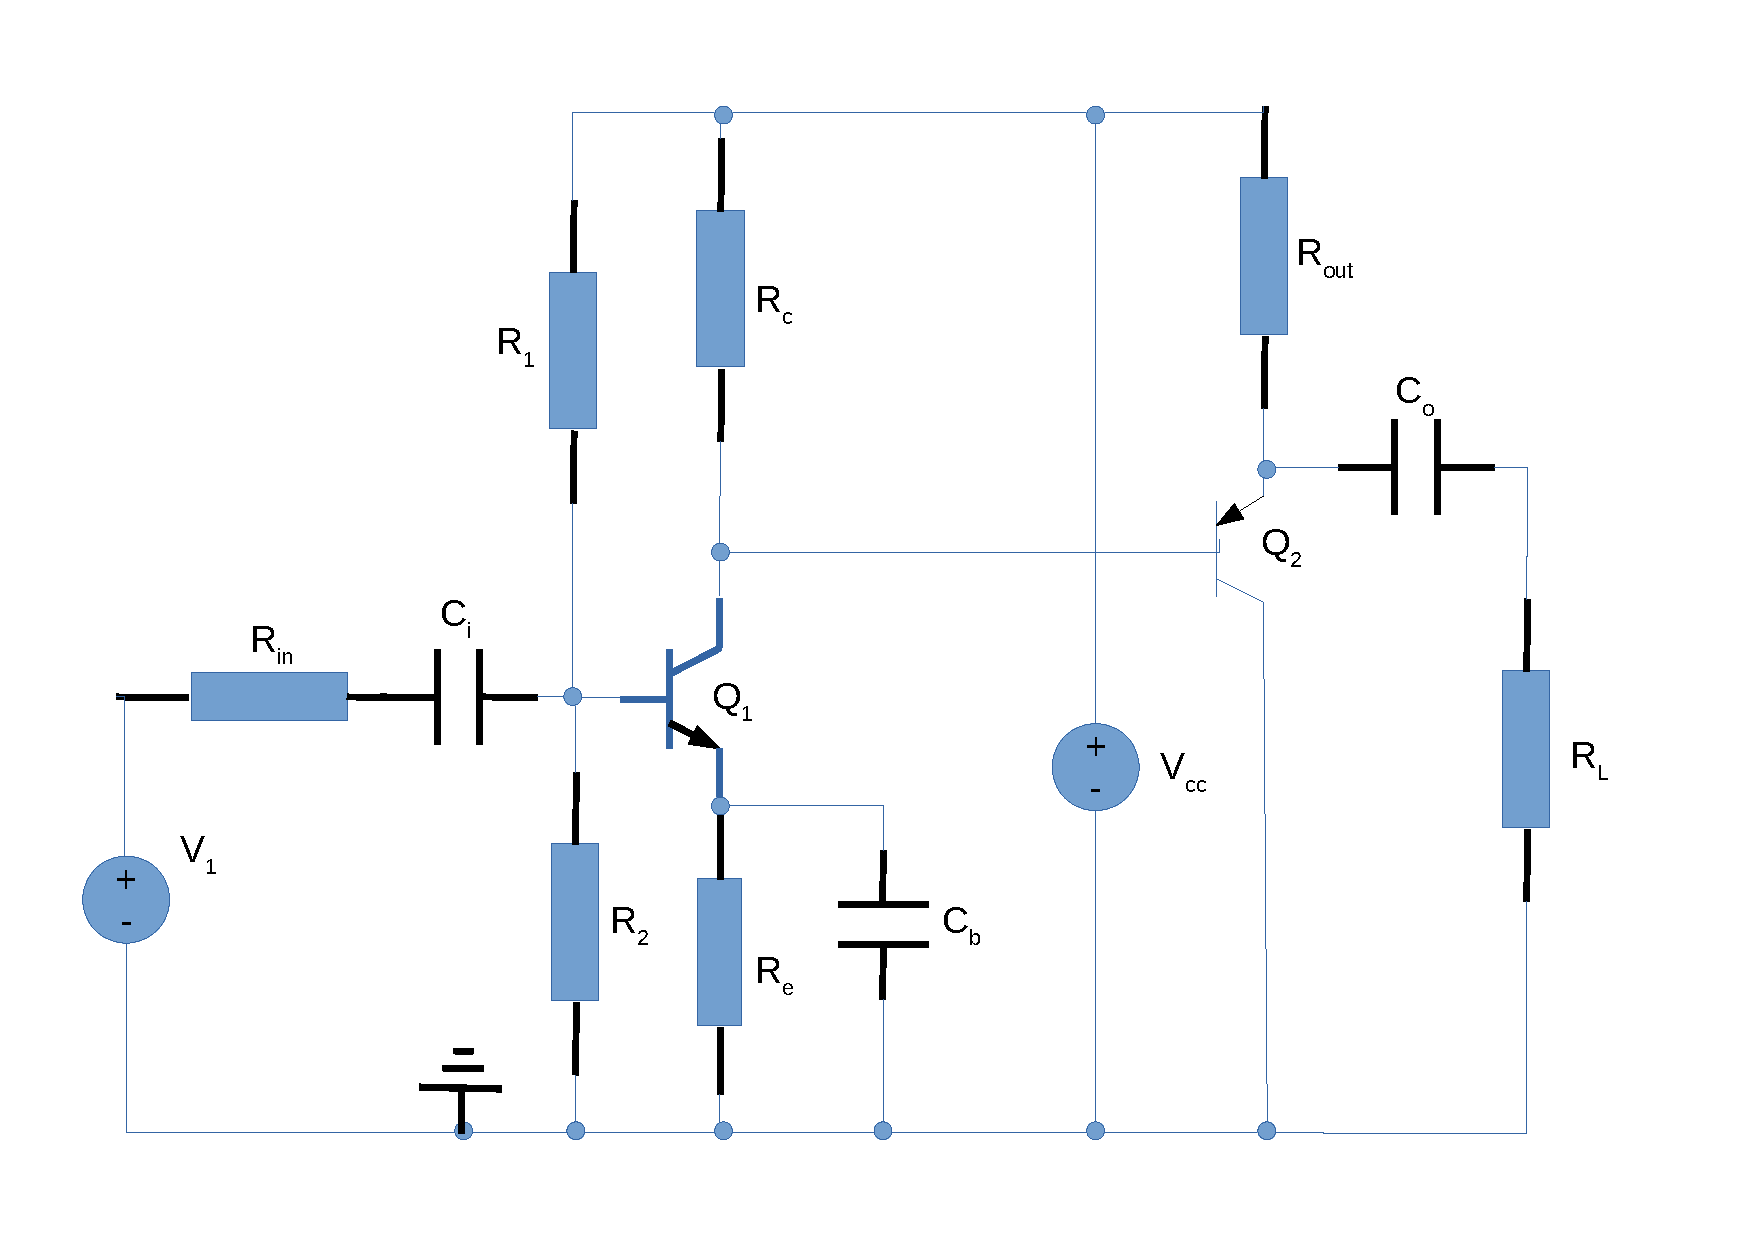
\includegraphics[width=0.85\linewidth]{dsnh_t4.pdf}
	\caption{Circuit T4}
\label{fig:Desenho_t4}
\end{figure}


